\chapter{Systems Engineering Methodological Approach}\label{app:se_approach}

\begin{figure}[H]
	\centering
	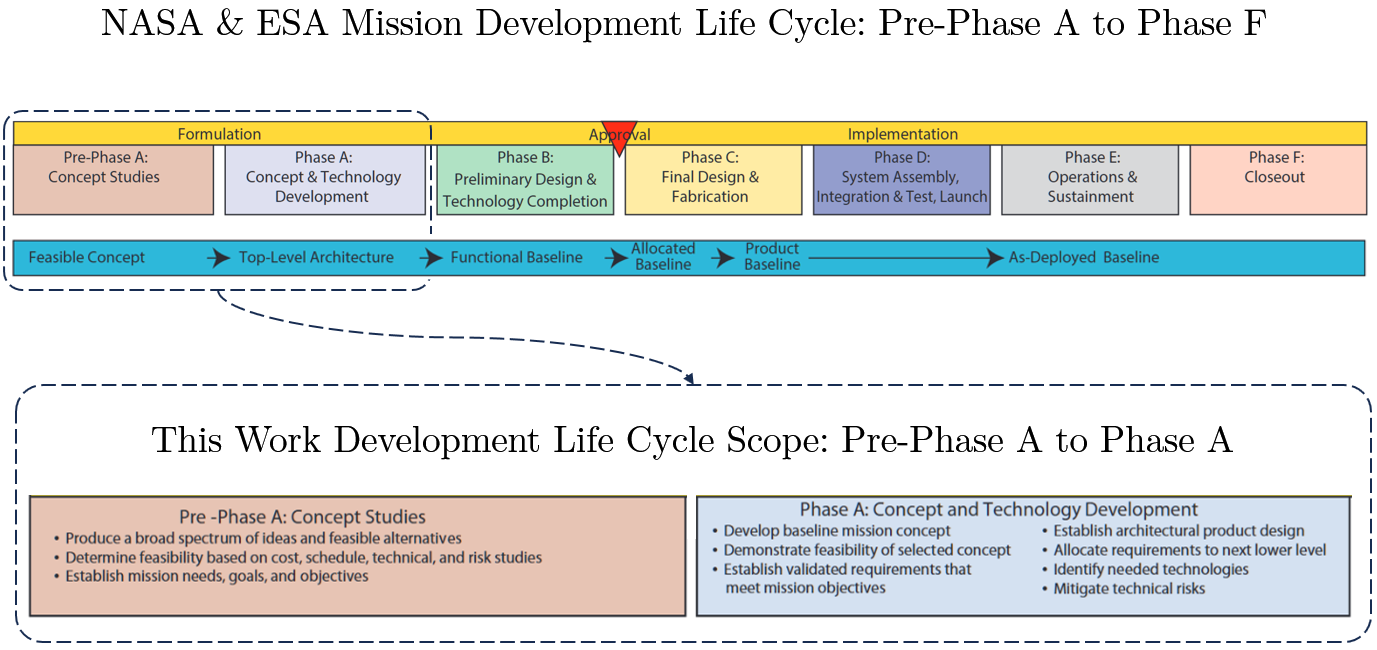
\includegraphics[width=1\textwidth]{images/c1.4_NASA_development_lifecycle.png}
	\caption[{NASA \& ESA Systems Engineering Development Life-Cycle. This work only covers Pre-Phase A and Phase A. Adapted from}]{NASA \& ESA Systems Engineering Development Life-Cycle. This work only covers Pre-Phase A and Phase A. Adapted from \parencite{SEHandbook}.}
	\label{fig:nasa-lifecycle}
\end{figure}

NASA's space-flight project life cycle is organized for complex product development involving multidisciplinary teams and disciplines \cite{SEHandbook}. As the mission development involves intricate requirements development, using a systems engineering approach enables this project to deliver a mission baseline solution in a scientific and systems engineering language, allowing further future work to be easily transferred and developed within engineering and other disciplines' frameworks. 

The scope of the SE life-cycle is summarized in Figure \ref{fig:nasa-lifecycle}. The life-cycle partitions work into discrete phases, separated by Key Decision Points (KDPs) where readiness to advance is assessed. Pre-Phase A (Concept Studies) surveys mission needs, feasibility, and trades and constraints. Phase A (Concept \& Technology Development) matures the mission concept, baselines initial system-level requirements, identifies technology gaps, establishes architectural product design, demonstrates the feasibility of the selected concept, and allocates requirements to the next lower system level. Phase B (Preliminary Design \& Technology Completion) completes technology maturation and the preliminary design. Phase C (Final Design \& Fabrication) finalizes detailed design and builds the flight system. Phase D (System Assembly, Integration \& Test, Launch \& Checkout) integrates and verifies the system and conducts launch/commissioning. Phase E (Operations \& Sustainment) conducts on-orbit operations, and Phase F (Closeout) decommissions and archives. 

The scope, methods, and results of this work are contained only in Pre-Phase A and Phase A, as these phases establish feasibility, architecture, and early requirements that drive all downstream design decisions.
